\documentclass[12pt]{article}
\usepackage[utf8]{inputenc}
\usepackage[spanish]{babel}

%Fuente (compilarlo en Latex.pdf normal porque va más rápido y luego
%y al final insertarlo en Arial) DA ERROR
%\usepackage{fontspec}
%\setmainfont{Arial}

%Estructura de la Página
\usepackage[left=2.54cm,right=2.54cm,top=2.54cm,bottom=2.54cm]{geometry}

%Páginas en horizontal


%Pies de página y encabezado
\usepackage{fancyhdr}

%Comentario párrafos
\usepackage{verbatim}

%Paquete arquitectura página
\pagestyle{fancy}
\fancyhf{}
\lhead{José Honrubia Blanco}
\rhead{Exámenes Ingeniería Térmica.}
\rfoot{\thepage}
\lfoot{Academia David Martínez}

%Interlineado
\renewcommand{\baselinestretch}{1}



%Paquete Matemático
\usepackage{amsmath}
\usepackage{amsfonts}
\usepackage{amssymb}
\usepackage{breqn}

%Paquete para el código
% Paquetes Listing

\usepackage{listings}
\usepackage{xcolor}

%Settings 

\definecolor{codegreen}{rgb}{0,0.6,0}
\definecolor{codegray}{rgb}{0.5,0.5,0.5}
\definecolor{codepurple}{rgb}{0.58,0,0.82}
\definecolor{backcolour}{rgb}{0.95,0.95,0.92}


\lstdefinestyle{mystyle}{
 backgroundcolor=\color{backcolour},   
 commentstyle=\color{codegreen},
 keywordstyle=\color{magenta},
 numberstyle=\tiny\color{codegray},
 stringstyle=\color{codepurple},
 basicstyle=\ttfamily\footnotesize,
 breakatwhitespace=false,         
 breaklines=true,                 
 captionpos=b,                    
 keepspaces=true,                 
 numbers=left,                    
 numbersep=5pt,                  
 showspaces=false,                
 showstringspaces=false,
 showtabs=false,                  
 tabsize=2
}

\lstset{style=mystyle}
%Paquete Imágenes

\usepackage{graphicx}
\usepackage{subcaption}
\graphicspath{ {imagenes/} }



%Bibliografía
\usepackage[backend=bibtex]{biblatex}
\addbibresource{referencias.bib}

%Espacio entre párrafos
\setlength{\parskip}{0.05cm}
%Sangría
\setlength{\parindent}{0cm}




\title{Exámenes Ingeniería Térmica}
\author{José Honrubia Blanco }
\date{Noviembre 2022}

\begin{document}

\section{Examen Octubre 2020}
\subsection{TEORÍA}
\textbf{Pregunta 1}. (1 punto) Un dispositivo cilindro-pistón de 24 $m^{3}$ contiene 8 kg de Helio a 288 K. Se suministra trabajo desde el exterior hasta que el volumen específico se reduce a 0.5 $\frac{m ^{3}}{kg}$ y la temperatura alcanza los 353 K. La temperatura ambiental es de 25 ºC. Calcular: la variación de exergía del Helio expresada en kJ. Considere los calores específicos del Helio constantes a tempertarua de 300 K y la presión ambiental 1 bar.
\\ 
\textbf{Pregunta 2}. (1 punto) Un flujo másico de $2 \frac{kg}{s}$ de vapor se expansiona de forma irreversible en una tobera que funciona en estado estacionario. El vapor entra en la tobera a 40 bar y 400 ºC y con una velocidad de 10 $\frac{m}{s}$. La tobera se puede considerar adiabática y la variación de energía potencial de vapor despreciable. A la salida la presión del vapor es de 14 bar y su velocidad es de $665 \frac{m}{s}$. Determine el área de la sección de salida de la tobera en $m ^{2}$.
\\
\textbf{Pregunta 3}. (1 punto) Un tanque rígido contiene agua a 16 $MPa$ y 360 ºC. Calcule:
\begin{itemize}
    \item El volumen específico del agua usando la ley de los gases.
    \item El volumen específico usando el factor de compresibilidad.
    \item El error que se comete usando las aproximadciones de los apartados anteriores.
\end{itemize}
\\
\textbf{Pregunta 4}. (1 punto)
\begin{itemize}
    \item La irradiación total sobre un cuerpo es de $2200 \frac{W}{m ^{2}}$. De esta cantidad, $450 \frac{W}{m ^{2}}$ los refleja y $900 \frac{W}{m ^{2}}$ los absorbe. Determine la transmisividad.
    \item La superficie de un cuerpo negro está a $115 ºC$. Determine la potencia emisiva espectral a la que la longitud de onda máxima $\frac{W}{m ^{2}\mu m}$
\end{itemize}

\subsection{PROBLEMAS}
\textbf{Problema 1}. (\textbf{2 puntos}) Un dispositivo cilindro-pistón contiene aire a 1250 $kPa$ y 60 ºC, el cual puede considerarse gas ideal con calores específicos constantes ($c _{P} = 1.005 \frac{kJ}{kg \cdot K}$, $C _{V} = 0.718 \frac{kJ}{kg \cdot K}$). El aire sufre un proceso de expansión hasta alcanzar los 140 $kPa$, el cual se puede considerar adiabático pero irreversible,, con un rendimiento isoentrópico de la expansión del 95\%. Considere el ambiente a 25 ºC y 1 bar. Determine:
\begin{itemize}
    \item Dibuje el diagrama T-s de la transformación y halle la temperatura final K de la misma.
    \item La variación de exergía específica que sufre el aire en $\frac{kJ}{kg}$.
    \item El trabajo útil específico en $\frac{kJ}{kg}$.
    \item La eficiciencia exergética de la expansión y energía disponible perdida específica en $\frac{kJ}{kg}$.
\end{itemize}

\textbf{Problema 2}. (\textbf{2 puntos}) Un motor de 4 tiempos y 4 cilindros realiza un ciclo ideal Otto. Se conocen los siguientes datos:
\begin{table}[h]
    \begin{tabular}{ll|ll}
    \hline
    \textbf{Carrera Pistón}          & 40 mm        & \textbf{Diámetro Pistón}                  & 60 mm  \\
    \textbf{Rendimiento Volumétrico} & 0.9          & \textbf{Rendimiento Mecánico}             & 0.8    \\
    \textbf{Relación de compresión}  & 12           & \textbf{Presión de admisión}              & 1 bar  \\
    \textbf{Coeficiente adiabático}  & 1.4          & \textbf{Presión media indicada}           & 15 bar \\
    \textbf{Dosado}                  & 20           & \textbf{Poder calorífico del combustible} & 45000  \\
    \textbf{Velocidad angular}       & 1600 rev/min & \textbf{Densidad del aire}                & 1.293  \\ \hline
    \end{tabular}
\end{table}

Determine:
\begin{itemize}
    \item Las presiones y volúmenes de cada punto del ciclo.
    \item La potencia efectiva.
    \item El par efectivo.
    \item La velocidad media del émbolo
\end{itemize}

\textbf{Problema 3}. (\textbf{2 puntos}) En la figura se esquematiza una sección de 1 m de caldera diseñada para suministrar agua de calefacción a un edificio de 50 viviendas. El cuerpo de la caldera, cuya resistencia térmica es despreciable, está fabricado en hierro fundido (negro en la imagen) y está aislado exteriormente mediante un calorifugado de lana de roca. Determine:
\begin{itemize}
    \item El flujo de calor que se evacua hacia el exterior a través del calorifugado.
    \item La temperatura del cuerpo de la caldera $T _{cc}$.
    \item El flujo de calor radiante y de calor convetivo en el interior de la caldera.
    \item El flujo de calor que se evacua por el agua.
    \item La longitud que debería tener la caldera para suministrar 500 kW de calefacción.
\end{itemize}

\begin{figure}[!h]
    \centering
    \begin{subfigure}[b]{0.45 \linewidth}
    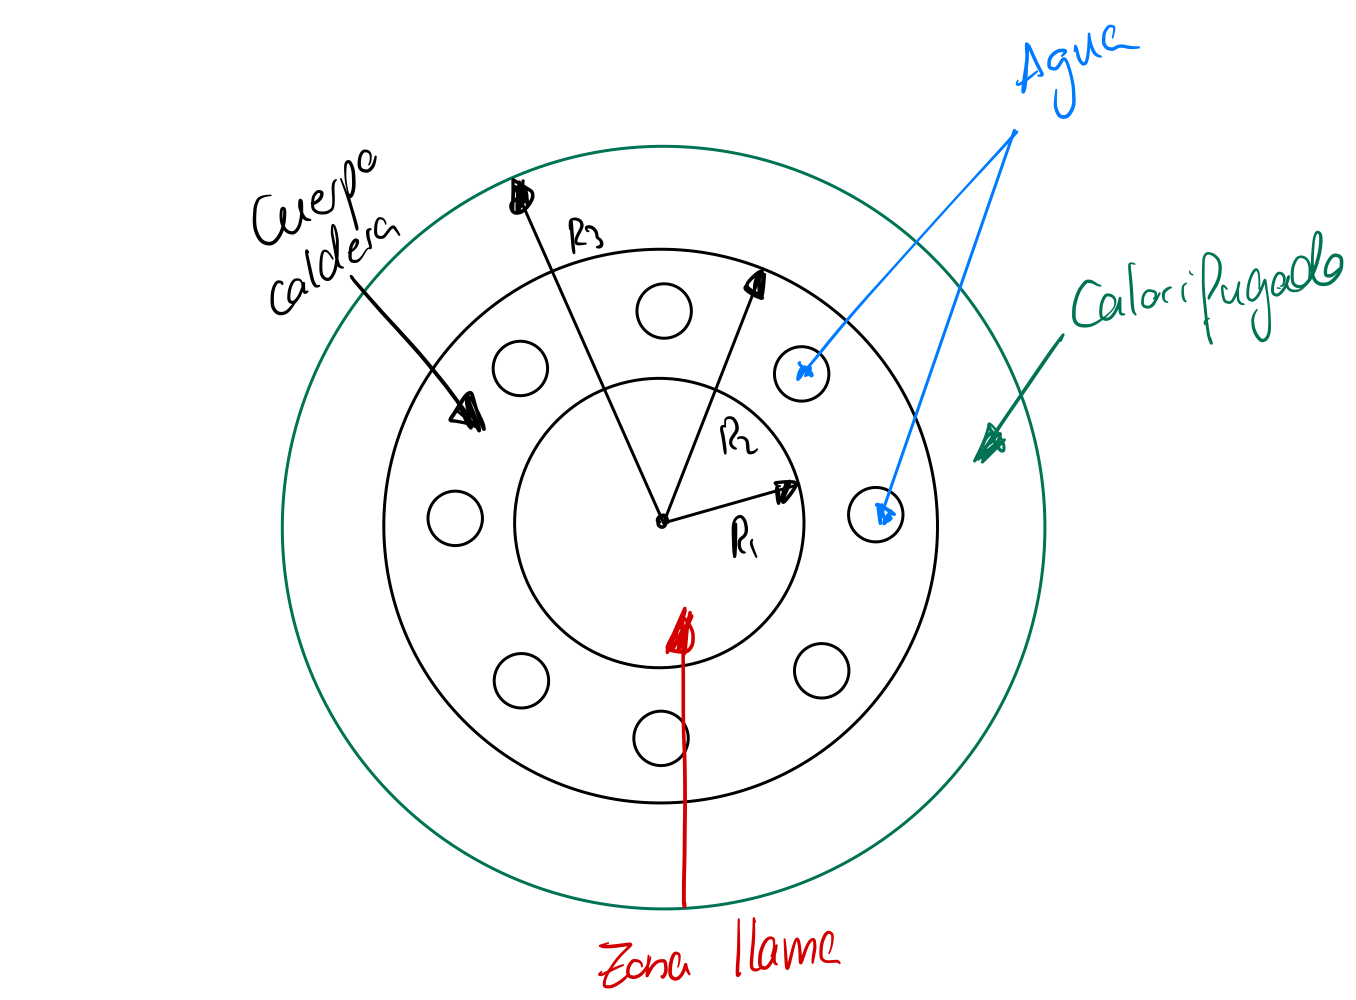
\includegraphics[width=\linewidth]{frontal_caldera.jpeg}
    \caption{Vista Frontal}
    \label{fig:westminster_lateral}
    \end{subfigure}
    \begin{subfigure}[b]{0.45 \linewidth}
    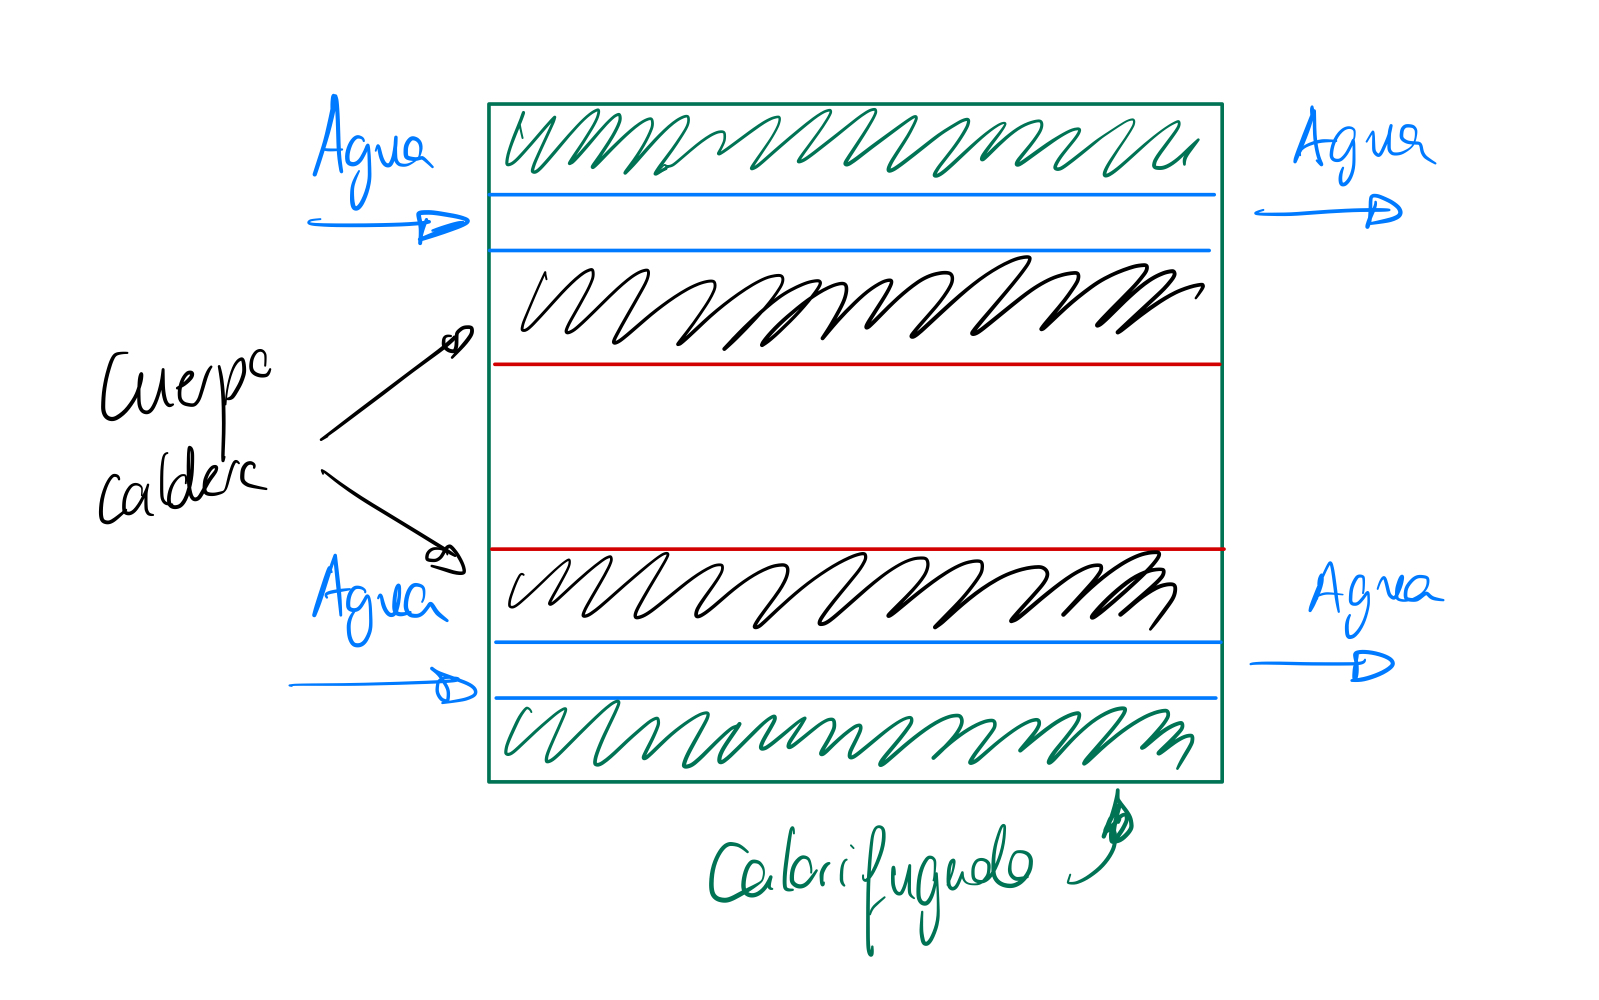
\includegraphics[width=\linewidth]{perfil_caldera.jpeg}
    \caption{Vista Lateral}
    \label{fig:westminster_aerea}
    \end{subfigure}
    \caption{Caldera}
    \label{fig:westminster}
   \label{fig:Caldera }
\end{figure}

Datos: $R _{1} = 0.3m$, $R _{2}=0.5m$, $R _{3}=0.6m$, $h _{e}= 12 \frac{W}{m ^{2}K}$, $h _{i}= 150 \frac{W}{m ^{2}K}$, $h _{r}= 60 \frac{W}{m ^{2}K}$, $k _{lana}= 0.05 \frac{W}{m ^{2}K}$, $T _{llama} = 1900$ ºC, $T _{i}= 700$ ºC, $T _{e}= 35$ ºC, $T _{0}= 25$ ºC.

\end{document}